%!TEX root = ../PhD_thesis__Lilian_Besson

% First chapter begins here
\chapter{Introduction}
\label{chapter:1}
\minitoc

\paragraph{Abstract.}
We start by presenting the problems studied in this thesis,
then we announce the different directions we considered and the solutions we proposed.
We give an overview of our main contributions, alongside a list of publications written in the last three years.

\newpage
% Write miniTOC just after the title
\graphicspath{{2-Chapters/1-Chapter/Images/}}

% ----------------------------------------------------------------------------
\section{Considered problems}
\label{sec:1:problems}

\TODOL{Write this!}

\subsection{Spectrum scarcity}


\subsection{Low-consumption IoT devices for the future}


% ----------------------------------------------------------------------------
\section{Considered solutions}
\label{sec:1:solutions}

\TODOL{Write this!}


\subsection{Online/sequential machine learning to automatically improve wireless communications on the run}

\subsection{Example: Opportunistic Spectrum Access (OSA) in licensed bands}

\subsection{Example: decentralized learning in unlicensed bands with selfish or orthogonalization-based MAB algorithms}


\subsection{Reinforcement learning}

\tikzstyle{block} = [align=center, draw, fill=gray!25, rectangle, minimum height=3em, minimum width=6em]
\begin{figure}[h!]
    \centering
    \resizebox{0.40\textwidth}{!}{
        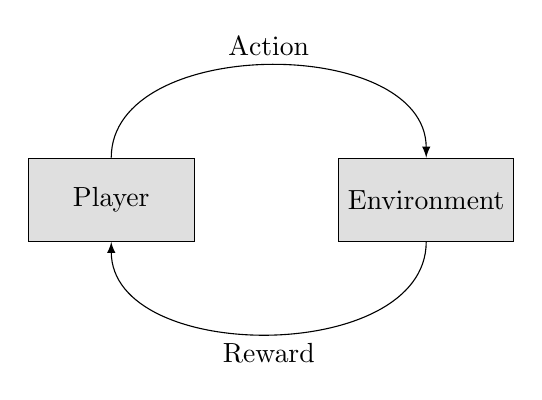
\begin{tikzpicture}[auto,node distance=5cm,>=latex,scale=2]
            %
            % We start by placing the blocks
            \node [block] (player) at (0,0) {Player};
            % We draw an edge between the player and system block to
            \node [block] (environment) at (2,0) {Environment};
            % Once the nodes are placed, connecting them is easy.
            \draw [->] (player) to[bend left=90] node[pos=0.5] {Action} (environment);
            \draw [->] (environment) to[bend left=90] node[pos=0.5] {Reward} (player);
            %
        \end{tikzpicture}
    }
\caption{Reinforcement learning cycle.}
\label{fig:1:ReinforcementLearningCycle}
\end{figure}


% ----------------------------------------------------------------------------
\section{Overview of the contributions}
\label{sec:1:contributions}

We can list the following points to summarize the main contributions of this thesis:

\begin{itemize}
    \item
    We present the concepts and the notations of the multi-armed bandit problem in Chapter~\ref{chapter:2}, from a mathematical point-of-view.
    But we also follow a didactic approach as we use an online interactive demonstration designed to let anyone play against a small bandit problem from his/her browser, in Section~\ref{par:2:interactiveDemoDiscoverMAB}.

    \item
    We give a short literature review of stochastic bandit algorithms in Section~\ref{sec:2:famousMABalgorithms}.

    \item
    We present the problem of choosing which algorithm a practitioner should use, or algorithm selection from the rich collection of different MAB available, in Section~\ref{sec:2:chooseYourPreferredBanditAlgorithm}.
    We present an algorithm called \Aggr{} for aggregation of algorithms as an online solution to the algorithm selection problem, and numerical simulations to illustrate that it achieves state-of-the-art empirical performances
    \cite{Besson2018WCNC}.
    % with \textbf{Aggregator} (WCNC 2018)

    \item
    We wrote the most complete open-source simulation library for MAB problems, called SMPyBandits, which is published online under an open-source licence \cite{SMPyBandits,SMPyBanditsJMLR}.
    We present in details its architecture and its features in Chapter~\ref{chapter:3}, along with different examples of its usage.
    A full documentation is available online, as well as exhaustive instructions to reproduce the experiments used in the rest of this thesis.

    \item
    We propose different models for IoT networks, in Chapter~\ref{chapter:4}, where end-devices with cognitive radio capabilities can implement MAB algorithms on their side, to automatically increase their battery life and allow more devices to use the same network while maintaining a high Quality of Service
    \cite{Bonnefoi17,Besson2019WCNC,Bonnefoi2019WCNC}.
    % (CROWNCOM 2017, ICT demo 2018, WCNC 2019 and MOTIoN 2019)

    \item
    We implemented a proof-of-concept of the aforementioned model \cite{Besson2018ICT}, and we present it in details in Section~\ref{sec:4:gnuradio}. We made a video showcasing our demonstration, hosted at \texttt{\href{https://youtu.be/HospLNQhcMk}{youtu.be/HospLNQhcMk}}.

    \item
    The source code for the two previously mentioned contributions are all published online, along with clear instructions for reproducing our work.

    \item
    We formalize the multi-player bandit model, and we introduced three variants, in Chapter~\ref{chapter:5}.
    For the case with sensing information, we propose two new algorithms, and we give an analysis for our algorithm \MCTopM{} to show it is order-optimal,
    as well as extensive numerical experiments to demonstrate its good performance in comparison with the rest of the literature.
    Our work \cite{Besson2018ALT} also gave a new impulse on research on multi-player bandits, as some recent research works built up on our results.

    \item
    We also give a detailed literature review of the different extensions of the multi-player MAB model, which we believe was never written before.
    % were  (ALT 2018, and 4-8 works inspired by our article since then). State-of-the-art with our algorithm MCTopM + klUCB for multi-player bandits "with sensing", empirical state-of-the-art with our simple (but wrong) "selfish" approach in case of "no sensing"

    \item
    We also present the piece-wise stationary MAB model, in Chapter~\ref{chapter:6}, and a detailed literature review of the research on non stationary MAB \cite{Besson2019GLRT,Besson2019Gretsi}.
    Following two recent works, we propose a new actively adaptive algorithm for the piece-wise stationary problem, \GLRklUCB, that achieves state-of-the-art performance.
    % - Literature review on non stationary models and algorithms, state-of-the-art for piece-wise stationary with our algorithm, GLR test + klUCB

    \item
    The last contribution of this thesis is a literature review of the possible use cases of the doubling trick technique for MAB problems,
    and a unified and more generic analysis of two families of doubling tricks.
    This lead to the article \cite{Besson2018DoublingTricks}, which is quickly presented in Appendix~\ref{app:2:DoublingTricks}, but not in the main text of the thesis.
\end{itemize}


% ----------------------------------------------------------------------------
\section{Organization of the thesis}
\label{sec:1:organization}

\begin{figure}[h!]
    \centering
    % \resizebox{1.00\textwidth}{!}{
    \begin{tikzpicture}[>=latex',line join=bevel,scale=2.25]
        %
        \node[align=center] (introduction) at (0,3.25) [rectangle,draw] {Chapter~\ref{chapter:1}\\Introduction};
        \node[align=center] (chapter2) at (0,2.25) [rectangle,draw] {Chapter~\ref{chapter:2}\\Stochastic and Stationary\\Multi-Armed Bandit models};
        \node[align=center] (chapter3) at (2.5,2.25) [rectangle,draw] {Chapter~\ref{chapter:3}\\SMPyBandits: simulation\\library for MAB};
        \node[align=center] (chapter4) at (-2.5,1) [rectangle,draw] {Chapter~\ref{chapter:4}\\Two MAB models\\for IoT networks};
        \node[align=center] (chapter5) at (0,1) [rectangle,draw] {Chapter~\ref{chapter:5}\\Multi-players\\MAB models};
        \node[align=center] (chapter6) at (2.5,1) [rectangle,draw] {Chapter~\ref{chapter:6}\\Non-stationary\\MAB models};
        \node[align=center] (conclusion) at (0,-0.25) [rectangle,draw] {Chapter~\ref{chapter:conclusion}\\General conclusion};
        %
        \draw [color=black,thick,->] (introduction) to (chapter2);
        \draw [color=black,thick,<->] (chapter2) to (chapter3);
        \draw [color=black,thick,->] (chapter2) to (chapter4);
        \draw [color=black,thick,->] (chapter2) to (chapter5);
        \draw [color=black,densely dotted,<->]   (chapter4) to (chapter5);
        \draw [color=black,densely dotted,->] -| (chapter3) to (chapter6);
        \draw [color=black,densely dotted,<->]   (chapter5) to (chapter6);
        \draw [color=black,thick,->] (chapter2) to (chapter6);
        \draw [color=black,thick,->] (chapter4) to (conclusion);
        \draw [color=black,thick,->] (chapter5) to (conclusion);
        \draw [color=black,thick,->] (chapter6) to (conclusion);
        %
    \end{tikzpicture}
    % }
    \caption{Organization of the thesis: a reading map. Any path containing Chapter~\ref{chapter:1}, Chapter~\ref{chapter:2}, at least one of the three Chapters~\ref{chapter:4}, \ref{chapter:5} and \ref{chapter:6}, and the Conclusion is a self contained way to read this thesis.}
    \label{fig:1:organization}
\end{figure}

The reading order of the manuscript can be any top-down path between Chapter~\ref{chapter:1} and the Conclusion in Chapter~\ref{chapter:conclusion}, in the graph shown in Figure~\ref{fig:1:organization} above,
and the thesis is organized in two parts:

In Part~\ref{part:Introduction}, we start by the next Chapter~\ref{chapter:2} where we introduce the MAB models, the concepts and the notations used in all this document, and it is mandatory to read it.
Conversely, Chapter~\ref{chapter:3} presents our simulation library SMPyBandits, and even if Chapters~\ref{chapter:2}, \ref{chapter:5} and \ref{chapter:6} use the library for their numerical simulation, reading this chapter is not required to understand the rest of the document.

Then the second Part~\ref{part:MABIOT} contain three chapters, that are included in both the logical and chronological orders, but can be read almost independently.
Chapter~\ref{chapter:4} starts by presenting different models of IoT networks where MAB algorithms have been used with success. Our two models are interesting and close to reality, but they appeared to be too general to propose a mathematical analysis of the good empirical performance of the considered solutions.
For this reason, we weaken the models for the rest of the document,
and both Chapters~\ref{chapter:5} and \ref{chapter:6} studies an intermediate model, lying between the stationary single-player MAB model from Chapter~\ref{chapter:2} and the IoT networks models from Chapter~\ref{chapter:4}.


% ----------------------------------------------------------------------------
\section{List of publications}
\label{sec:1:listPublications}

% =============================================================================
\subsection{Publications in international conferences with proceedings}

\begin{itemize}

\item
    \emph{Decentralized Spectrum Learning for IoT Wireless Networks Collision Mitigation},\\
    by Christophe Moy \& \textbf{Lilian Besson}.
    1st International ISIoT workshop\footnote{~See \href{https://sites.google.com/view/ISIoT2019}{\texttt{sites.google.com/view/ISIoT2019}}},
    at \emph{Conference on Distributed Computing in Sensor Systems}\footnote{~IEEE DCOSS 2019, see \href{http://2019.dcoss.org}{\texttt{2019.dcoss.org}}}, Santorini, Greece, May 2019.
    \cite{MoyBesson2019}

\item
    \emph{Upper-Confidence Bound for Channel Selection in LPWA Networks with Retransmissions},\\
    by Rémi Bonnefoi, \textbf{Lilian Besson}, J. Manco-Vasquez \& Christophe Moy.
    1st International MOTIoN workshop\footnote{~MOTIoN 2019, see \href{https://sites.google.com/view/wcncworkshop-motion2019}{\texttt{sites.google.com/view/wcncworkshop-motion2019}}},
    at \emph{IEEE WCNC}, Marrakech, Morocco, April 2019.
    \cite{Bonnefoi2019WCNC}

\item
    \emph{GNU Radio Implementation of MALIN: ``Multi-Armed bandits Learning for Internet-of-things Networks''},
    by \textbf{Lilian Besson}, Rémi Bonnefoi \& Christophe Moy.
    \emph{Wireless Communication and Networks Conference}\footnote{~IEEE WCNC 2019, see \href{http://wcnc2019.ieee-wcnc.org}{\texttt{wcnc2019.ieee-wcnc.org}}}, Marrakech, Morocco, April 2019,
    \href{https://HAL.Inria.fr/hal-02006825}{\texttt{HAL.Inria.fr/hal-02006825}}.
    \cite{Besson2019WCNC}

\item
    \emph{Multi-Player Bandits Revisited},
    by \textbf{Lilian Besson} \& Emilie Kaufmann.
    \emph{Algorithmic Learning Theory}\footnote{~ALT 2018, see \href{http://www.cs.cornell.edu/conferences/alt2018}{\texttt{www.cs.cornell.edu/conferences/alt2018}}}, Lanzarote, Spain, April 2018,
    \href{https://HAL.Inria.fr/hal-01629733}{\texttt{HAL.Inria.fr/hal-01629733}}.
    \cite{Besson2018ALT}

\item
    \emph{Aggregation of Multi-Armed Bandits learning algorithms for Opportunistic Spectrum Access},\\
    by \textbf{Lilian Besson}, Emilie Kaufmann \& Christophe Moy.
    \emph{Wireless Communication and Networks Conference}\footnote{~IEEE WCNC 2018, see \href{http://wcnc2018.ieee-wcnc.org}{\texttt{wcnc2018.ieee-wcnc.org}}}, Barcelone, Spain, April 2018,
    \href{https://HAL.Inria.fr/hal-01705292}{\texttt{HAL.Inria.fr/hal-01705292}}.
    \cite{Besson2018WCNC}

\item
    \emph{Multi-Armed Bandit Learning in IoT Networks and non-stationary settings},
    by Rémi Bonnefoi, \textbf{Lilian Besson}, Christophe Moy, Emilie Kaufmann \& J. Palicot.
    \emph{Conference on Cognitive Radio Oriented Wireless Networks}\footnote{~CROWNCOM, \href{http://crowncom.org/2017}{\texttt{crowncom.org/2017}}}, Lisboa, Portugal, Septembre $2017$,\\
    \href{https://HAL.Inria.fr/hal-01575419}{\texttt{HAL.Inria.fr/hal-01575419}},
    \textbf{Best Paper Award}.
    \cite{Bonnefoi17}

\end{itemize}

% =============================================================================
\subsection{Demonstration in international conferences}

\begin{itemize}

\item
    \emph{MALIN: ``Multi-Arm bandit Learning for Iot Networks'' with GRC: A TestBed Implementation and Demonstration that Learning Helps},
    by \textbf{Lilian Besson}, Rémi Bonnefoi, Christophe Moy.
    Demonstration presented at \emph{International Conference on Communication}\footnote{~ICT, \href{http://ict-2018.org/demos}{\texttt{ict-2018.org/demos}}}, in Saint-Malo, France in June $2018$.
    See \href{https://YouTu.be/HospLNQhcMk}{\texttt{YouTu.be/HospLNQhcMk}} for a $6$-minutes presentation video.
    \cite{Besson2018ICT}

\end{itemize}


% =============================================================================
% \subsection{French language conference with proceedings}
\subsection{Submitted works}

\begin{itemize}
\item
    \emph{Analyse non asymptotique d'un test séquentiel de détection de ruptures et application aux bandits non stationnaires} (in French),
    submitted at GRETSI 2019\footnote{~\href{http://GRETSI.fr/colloque2019}{\texttt{GRETSI.fr/colloque2019}}},
    by \textbf{Lilian Besson} \& Emilie Kaufmann, March $2019$,
    \href{https://HAL.Inria.fr/hal-02006471}{\texttt{HAL.Inria.fr/hal-02006471}}.
    \cite{Besson2019Gretsi}

\end{itemize}


% =============================================================================
\subsection{In progress works waiting for a new submission}

\begin{itemize}

\item
    \emph{The Generalized Likelihood Ratio Test meets klUCB: an Improved Algorithm for Piece-Wise Non-Stationary Bandits},
    by \textbf{Lilian Besson} \& Emilie Kaufmann, \\
    February $2019$,
    \href{https://HAL.Inria.fr/hal-02006471}{\texttt{HAL.Inria.fr/hal-02006471}}.
    \cite{Besson2019GLRT}

\item
    \emph{SMPyBandits: an Open-Source Research Framework for Single and Multi-Players Multi-Arms Bandits (MAB) Algorithms in Python},
    by \textbf{Lilian Besson}, active development since October $2016$,
    \href{https://HAL.Inria.fr/hal-01840022}{\texttt{HAL.Inria.fr/hal-01840022}}.
    About $40000$ lines of code, hosted on \href{https://GitHub.com/SMPyBandits}{\texttt{GitHub.com/SMPyBandits}},
    and documentation on \href{https://SMPyBandits.rtfd.io}{\texttt{SMPyBandits.rtfd.io}}.
    \cite{SMPyBandits,SMPyBanditsJMLR}

\item
    \emph{What Doubling-Trick Can and Can't Do for Multi-Armed Bandits},
    by \textbf{Lilian Besson} \& Emilie Kaufmann,\\
    September $2018$,
    \href{https://HAL.Inria.fr/hal-01736357}{\texttt{HAL.Inria.fr/hal-01736357}}.
    \cite{Besson2018DoublingTricks}

\end{itemize}


% =============================================================================
\subsection{Other works}

\begin{itemize}
\item
    \emph{A Note on the Ei Function and a Useful Sum-Inequality},
    by \textbf{Lilian Besson},
    February $2018$,
    \href{https://HAL.Inria.fr/hal-01847480}{\texttt{HAL.Inria.fr/hal-01847480}}.

\end{itemize}


% =============================================================================
\subsection{Presentations in seminars and conferences}

\paragraph{Seminars}
    I gave some presentations in the following events:
    SequeL team seminar at Inria Lille in September and December $2017$, and June $2019$;
    SCEE team seminar at CentraleSupélec, Rennes campus, in October $2017$, February $2018$ and June $2019$;
    as well as
    for the GDR ISIS day held in Issy-les-Moulineaux on November $2017$,
    for the brown-bag seminar at ENSAI in Bruz in January $2018$,
    for the weekly seminar at CMAP lab at École Polytechnique in October $2018$,
    for the weekly seminar of the PANAMA project-team at IRISA / Inria Rennes in May $2019$.

\paragraph{Tutorial}
    I gave a tutorial on the Julia language, at IETR seminar in Vannes in June $2018$,
    with Pierre Haessig (\texttt{pierreh.eu}), see \href{https://HAL.Inria.fr/cel-01830248}{\texttt{HAL.Inria.fr/cel-01830248}}.

\paragraph{Training}
    I was also in charge of ``GouTP'' training sessions for about $30$ PhD students at CentraleSupélec Rennes.
    We had a lot of various $1$h training sessions between January $2017$ and June $2019$,
    and I gave about $12$ training sessions, on various topics including Python, \texttt{git}, HAL and arXiv, the Julia language and Bib\TeX{}.


% =============================================================================
\subsection{Other experiences}

\paragraph{Conferences}
    I attended the following conferences:
	\emph{International Conference on Communication} ICC (Paris), May $2017$,
    \emph{Conference on Learning Theory} COLT (Amsterdam), July $2017$,
    \emph{Conference on Cognitive Radio Oriented Wireless Networks} CROWNCOM (Lisboa), September $2017$,
    \emph{Conference on Algorithmic Learning Theory} ALT (Lanzarote), April $2018$,
    \emph{Wireless Communication and Networking Conference} WCNC (Barcelona), April $2018$,
	\emph{International Conference on Telecommunication} ICT (Saint-Malo), June $2018$,
    \emph{Wireless Communication and Networking Conference} WCNC (Marrakech), April $2019$,
    \emph{Colloque francophone de traitement du signal et des images} GRETSI (Lille), August $2019$.

\paragraph{Seminars}
    I attended the following seminars:
	\emph{Workshop Learn with Earning} (Rotterdam), May $2018$,
	\emph{Workshop on Optimization and Learning} (Toulouse), September $2018$,
	\emph{European Workshop on Reinforcement Learning} (Lille), October $2018$,

\paragraph{Responsabilities}
    I was the president of the PhD Students Association of IETR lab (ADDI, \texttt{addi.asso.insa-rennes.fr}) in $2017$.
    I was notably in charge of organizing the PhD Students day at Rennes, in June $2017$, with about $350$ people, and presentation of a research poster\footnote{~See \href{https://HAL.Inria.fr/hal-02013839}{\texttt{HAL.Inria.fr/hal-02013839}}}
    I also helped for the organization and presented another poster\footnote{~See \href{https://HAL.Inria.fr/hal-02013847}{\texttt{HAL.Inria.fr/hal-02013847}}} at the ``IETR : Interagir Évaluer Transmettre Réunir'' seminar, held in Vannes in June $2018$.

\paragraph{Reviews}
	for \emph{European Workshop on Reinforcement Learning}\footnote{~EWRL 2018, see \href{https://ewrl.wordpress.com/ewrl14-2018}{\texttt{ewrl.wordpress.com/ewrl14-2018}}} (Lille), in October $2018$, I reviewed $5$ papers.
	I helped colleagues for articles submitted at international conferences \emph{AISTATS} $2019$, \emph{NeurIPS} $2017$ et $2018$, and \emph{COLT} $2018$ and $2019$, for about 10 \emph{reviews}.

\paragraph{System Administrator}
	maintaining our workstations running GNU/Linux and Windows
	at SCEE team,
	and our cognitive radio test-bed using USRP cards and the GNU Radio software,
	from January $2017$ to September $2018$.

